\documentclass{ximera}

\title{Function Extrema Activity Solution Guide}
\author{MATH 425: Calculus I}

\begin{document}
\begin{abstract}
   Working with the peers in your group, solve the following problems. Make sure to show and justify all your work. Make sure everyone in the group understands the solution and participates. Be prepared to report your answers to the whole class. 
\end{abstract}
\maketitle


\begin{exercise}
    Sketch the graph of a function with domain $[-3,3]$ with the following: 
    \begin{itemize}
        \item local minima at $x=-2, 2$
        \item local maximum at $x=-3, 0$
        \item absolute minimum at $x=-2$
        \item absolute maximum at $x=-3$.
        \item a critical number at $x=1$ that is neither a local maximum nor minimum.
    \end{itemize}

    \begin{image}
        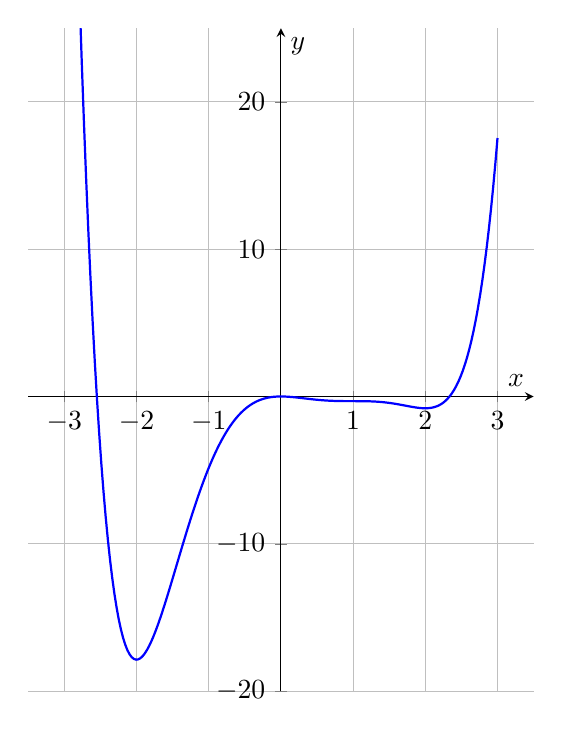
\begin{tikzpicture}
            \begin{axis}[
                xmin=-3.5, xmax=3.5,
                ymin=-20, ymax=25,
                xlabel=$x$,
                ylabel=$y$,
                grid=major,
                axis lines=middle,
                width=8cm,
                height=10cm
            ]
                \addplot[domain=-3:3, samples=200, thick, blue] {1/6*(x)^6-2/5*(x)^5-3/4*(x)^4+8/3*(x)^3-2*(x)^2};
            \end{axis}
        \end{tikzpicture}
    \end{image}
    %\xmalt{a graph of the function $f(x)=\frac{x^6}{6}-\frac{2x^5}{5}-\frac{3x^4}{4}+\frac{8x^3}{3}+2x^2$ on the interval $[-3,3]$.}
\end{exercise}

\begin{exercise}
    Find all critical numbers of the following functions: 
    \begin{enumerate}
        % \item $f(x)=x^3-4x^2+15x$ \\
        % \textcolor{blue}{ $f'(x)=3x^2-8x+15$\\
        % $f'(x)=0$ when $x=\frac{8\pm \sqrt{(-8)^2-4(3)(15)}}{2(3)}=$ no real solution\\
        % $f'$ always exists, since $f'(x)$ is a polynomial.\\
        % NO CRITICAL NUMBERS}
        
        \item $h(x)=\frac{x-1}{x^2+4}$\\
        \textcolor{blue}{ $h'(x)=\frac{(x^2+4)(1)-(x-1)(2x)}{(x^2+4)^2}=\frac{x^2+4-2x^2+2x}{(x^2+4)^2}=\frac{-x^2+2x+4}{(x^2+4)^2}$\\
        $f'(x)=0$ when $-x^2+2x+4=0$, so $x=\frac{-2\pm\sqrt{20}}{-2}$\\
        $f'$ DNE when $(x^2+4)^2=0$, or $x^2+4=0$, which has no real solution.\\
        Critical numbers: $x=0,1\pm\frac{\sqrt{20}}{-2} $.}
        
        \item $f(x)=x^{-2}\ln(x)$ for the domain $(0,\infty)$\\
        \textcolor{blue}{$f'(x)=x^{-2}(\frac{1}{x})+\ln(x)(-2x^{-3})=\frac{1}{x^3}-\frac{2\ln(x)}{x^3}=\frac{1-2\ln(x)}{x^3}$\\
        $f'(x)=0$ when $1-2\ln(x)=0$\\
        $1=2\ln(x)$\\
        $\frac{1}{2}=\ln(x)$\\
        $x=e^{\frac{1}{2}}$\\
        $f'$ DNE when $x^3=0$, or $x=0$, which is not in the domain.\\
        Critical Numbers: $x=e^{\frac{1}{2}}$}     
    \end{enumerate}
\end{exercise}

\begin{exercise}
    Identify the absolute maxima and minima of the function on the following interval \textbf{using the critical numbers of the functions}.
    \begin{enumerate}
        \item $f(x)=-2x^3+54x+5$ on $[0,4]$\\
        \textcolor{blue}{ Identify critical numbers: $f'(x)=-6x^2+54$\\
        $f'$ exists everywhere because it is a polynomial.\\
        $f'(x)=0$ when $-6x^2+54=0$\\
        $6x^2=54$\\
        $x^2=9$ so $x=3, -3$.  Only $x=3$ is in the interval we care about.\\
        $f(0)=-2(0)^3+54(0)+5=5 \leftarrow $ Abs min of $5$ at $x=0$\\
        $f(3)=-2(3)^3+54(3)+5=113 \leftarrow$ Abs max of $113$ at $x=3$\\
        $f(4)=-2(4)^3+54(4)+5=93$}
        
        \item $g(x)=x^2-4x-17$ on $[-1,5]$\\
        \textcolor{blue}{ Identify critical numbers: $f'(x)=2x-4$\\
        $f'$ exists everywhere because it is a polynomial\\
        $f'(x)=0$ when $2x-4=0$, or $x=2$.\\
        $f(-1)=(-1)^2-4(-1)-17=-12$\\
        $f(2)=(2)^2-4(2)-17=-21\leftarrow$ Abs min at $(2,-21)$\\
        $f(5)=(5)^2-4(5)-17=-12$\\
        Absolute max of $-12$ at both $x=-1, 5$}
        
        \item $h(x)=\sqrt{x}(x-1)$ on $[0,9]$\\
        \textcolor{blue}{ $h'(x)=x^{\frac{1}{2}}+\frac{1}{2}x^{-\frac{1}{2}}(x-1)=\frac{2x+x-1}{2x^{1}{2}}$\\
        $h'(x)=0$ when $3x-1=0$, or $x=\frac13$\\
        $h'$ does not exist when $2\sqrt{x}=0$ or $x=0$\\
        $h(0)=\sqrt{0}(0-1)=0$\\
        $h(\frac{1}{3})=\sqrt{\frac{1}{3}}(\frac{1}{3}-1)=\sqrt{\frac{1}{3}}(-\frac23)$\\
        $h(9)=\sqrt{9}(9-1)=3(8)=24$\\
        Absolute max of $24$ at $x=9$ and absolute min of $-\sqrt{\frac13}(\frac23)$ at $x=\frac{1}{3}$}
    \end{enumerate}
\end{exercise}




\end{document}
